% ============================================================
% Gradual Convergence, Not Discrete Breaks:
% Bitcoin's Volatility Under Institutional Adoption
% ============================================================
\documentclass[12pt,a4paper]{article}

% --- Packages ---
\usepackage[utf8]{inputenc}
\usepackage[T1]{fontenc}
\usepackage[margin=1in]{geometry}
\usepackage{amsmath,amssymb,amsthm,mathtools}
\usepackage[authoryear,round]{natbib}
\usepackage{booktabs}
\usepackage{tabularx}
\usepackage{graphicx}
\usepackage{float}
\usepackage{setspace}
\usepackage{xcolor}
\usepackage{threeparttable}
\usepackage{multirow}
\usepackage{siunitx}
\usepackage{placeins}
\usepackage{hyperref}
\hypersetup{hidelinks}
\usepackage{doi}

\raggedbottom

% --- Operators ---
\DeclareMathOperator*{\argmax}{arg\,max}
\DeclareMathOperator*{\argmin}{arg\,min}
\DeclareMathOperator{\Var}{Var}
\DeclareMathOperator{\Cov}{Cov}
\DeclareMathOperator{\plim}{plim}
\DeclareMathOperator{\sgn}{sgn}

% --- Figure path ---
\graphicspath{{figures/}}

\doublespacing

% ============================================================
\title{Cinderella at Midnight: \\ Bitcoin's Fragile Convergence to Traditional-Asset Volatility}

\author{E2ER by Bj\"{o}rn Hanneke%
\footnote{This manuscript has been AI-generated by the End-to-End-Researcher
(E2ER) pipeline, set up by Bj\"{o}rn Hanneke (hanneke@wiwi.uni-frankfurt.de).
Full replication package available upon request.}}

\date{\today}

\begin{document}

\maketitle

% ============================================================
\begin{abstract}
\noindent
Bitcoin's average volatility has converged toward traditional asset levels,
but this convergence is fragile. Using daily data on Bitcoin and seven
traditional benchmarks from 2020 to 2026, we show that Bitcoin's
unconditional GARCH volatility fell from 89 percent before the January 2024
spot ETF approval to 50 percent afterward, and that Markov-switching models
identify a low-volatility regime at 32 percent---within the range of
commodity volatility. The critical finding is that Bitcoin sustains this
calm regime for only six days on average, compared to 82 days for equities
and over 200 days for small-cap stocks. A cross-asset difference-in-differences
design finds no discrete structural break at the ETF date, and a
Mann-Kendall trend test confirms that the convergence is gradual rather
than event-driven. Bitcoin can reach traditional-asset volatility levels,
but institutional infrastructure has not yet provided the stabilization
needed to keep it there.
\\[6pt]
\textbf{JEL codes:} G12, G14, G18, C58 \\
\textbf{Keywords:} Bitcoin, realized volatility, institutional adoption, regime switching, GARCH, ETF, fragile convergence
\end{abstract}



% ============================================================
\section{Introduction}\label{sec:intro}
% ============================================================

Few assets have undergone as rapid a transformation in investor composition
as Bitcoin. In 2017, Bitcoin traded almost exclusively on unregulated
exchanges, held by retail investors with no access to institutional custody,
regulated derivatives, or index-fund wrappers. By early 2026, Bitcoin is
held in exchange-traded funds managing over \$100 billion in assets, traded
via CME futures with daily volumes exceeding \$5 billion, and incorporated
into the portfolio allocation frameworks of pension funds, endowments, and
sovereign wealth vehicles. This transition from retail curiosity to
institutional asset class occurred within a single decade---far faster than
the comparable institutionalization of gold, commodities, or real estate
investment trusts.

A central question for both investors and regulators is whether this
institutional adoption has changed Bitcoin's risk characteristics. Bitcoin's
annualized realized volatility averaged 57 percent over 2020--2026, roughly
three times the level of the S\&P~500 and nearly five times that of
investment-grade bonds. Yet this headline figure masks a pronounced downward
trajectory: the ratio of Bitcoin's realized volatility to traditional
benchmarks fell by approximately 15 percent over the same window, and the
decline shows no sign of reversal. Understanding whether this convergence
reflects institutional participation---or merely the passage of time as the
asset matures---matters for portfolio construction, derivative pricing, and
the regulatory classification of Bitcoin as an investable asset class.

The January 2024 approval of spot Bitcoin exchange-traded funds in the
United States provides a natural testing ground. Within months of approval,
cumulative net inflows into spot Bitcoin ETFs exceeded those of gold ETFs
during their first year of trading. Our conceptual framework identifies
three channels through which institutional participation could reduce
volatility: improved liquidity provision, more efficient information
aggregation, and expanded arbitrage capacity that dampens deviations from
fundamental value \citep{kyle1985continuous, grossman1980impossibility,
shleifer1997limits}. If these channels operate, the ETF launch should
produce a measurable reduction in Bitcoin's excess volatility relative to
assets unaffected by the event.

Prior work on Bitcoin volatility has established that GARCH and
Markov-switching models capture Bitcoin's conditional heteroskedasticity
\citep{katsiampa2017volatility, dyhrberg2016bitcoin, conrad2018long,
ardia2019regime, caporale2019modelling}, and a smaller literature has
examined the effect of specific institutional events on Bitcoin's price
dynamics \citep{augustin2023causal, kochling2019futures}. The emerging
post-2024 literature studies ETF-related changes in market microstructure
\citep{mazur2025spot, kia2025price, hong2025bitcoin, lee2025shifting}.
What is missing from this body of work is a characterization of Bitcoin's
volatility \emph{relative to traditional benchmarks}: not just whether
Bitcoin's volatility has declined, but whether it has converged toward
levels observed in established asset classes, whether that convergence is
durable, and what the regime structure of the convergence looks like.

Understanding Bitcoin's volatility trajectory matters beyond academic
curiosity. If institutional channels---liquidity, information efficiency,
and arbitrage capacity---are driving the convergence, then the pattern
should persist and potentially accelerate as institutional adoption
deepens. If instead the convergence reflects idiosyncratic market
conditions (the post-COVID recovery, the 2022 crypto winter), then
extrapolating the trend is unwarranted. Distinguishing between these
explanations has direct implications for the asset allocation decisions of
institutional investors, the margin requirements set by clearinghouses, and
the regulatory classification of Bitcoin under frameworks that condition on
volatility thresholds.

Against this background, we make three contributions. First, we document
what we call Bitcoin's \emph{fragile convergence}: GARCH(1,1) estimates
show that Bitcoin's unconditional volatility fell from 89 percent
(annualized) before the January 2024 ETF approval to 50 percent afterward,
and a Mann-Kendall trend test confirms a monotonic decline in the
BTC-to-traditional-asset volatility ratio over 2020--2026. Yet
Markov-switching models reveal that this convergence is skin-deep.
Bitcoin's low-volatility regime---at 32 percent annualized, within the
range of commodity volatility---persists for only six days on average,
compared to 82 days for equities and over 200 days for small-cap stocks.
Bitcoin can reach traditional-asset volatility levels; it cannot yet
sustain them.

Second, we test whether the convergence concentrates at the January 2024
ETF approval using a cross-asset difference-in-differences design with ten
assets and wild cluster bootstrap inference. We find no discrete structural
break: the point estimate is economically small and statistically
indistinguishable from zero. Pre-trend tests reject the parallel trends
assumption, indicating that Bitcoin's volatility was already declining
relative to traditional assets before the ETF event---consistent with
gradual convergence driven by accumulating institutional infrastructure
rather than a single regulatory shock.

Third, we provide a cross-asset parametric characterization that places
Bitcoin in the context of established asset classes. GARCH persistence is
comparable across all ten assets (0.94--0.99), suggesting that Bitcoin's
volatility process has the same memory structure as equities and bonds. The
key differentiator is regime fragility: the Markov-switching model shows
that traditional assets maintain low-volatility regimes for months, while
Bitcoin's calm is repeatedly interrupted. The absence of leverage effects
in Bitcoin (GJR-GARCH asymmetry is insignificant, unlike equities) further
distinguishes its volatility dynamics and suggests that different
mechanisms govern the tails of the return distribution.

The remainder of this paper proceeds as follows. Section~\ref{sec:framework}
outlines the conceptual framework linking institutional participation to
volatility regime dynamics. Section~\ref{sec:data} describes the data.
Section~\ref{sec:methodology} presents the empirical methodology.
Section~\ref{sec:results} reports the results.
Section~\ref{sec:discussion} discusses implications and limitations.
Section~\ref{sec:conclusion} concludes.

\FloatBarrier

% ============================================================
\section{Conceptual Framework}\label{sec:framework}
% ============================================================

Three channels link institutional participation to asset volatility. The
first operates through \emph{liquidity provision}. Institutional investors
and ETF-authorized market makers commit capital to continuous two-sided
quoting, narrowing bid-ask spreads and absorbing order flow that would
otherwise move prices. The market microstructure literature, beginning with
\citet{kyle1985continuous} and \citet{glosten1985bid}, establishes that
deeper markets exhibit lower price impact per unit of trade, which
mechanically reduces transitory volatility driven by order-flow imbalances.

The second channel operates through \emph{information efficiency}.
Institutional participants tend to be better resourced for fundamental
analysis and faster at incorporating public information into prices
\citep{barber2008attention}. As the share of informed trading increases,
prices adjust more rapidly to fundamental news and less to noise, reducing
the variance of returns attributable to delayed information incorporation.
\citet{makarov2020trading} document that cross-exchange arbitrage in
Bitcoin markets tightened substantially over 2017--2018 as institutional
infrastructure improved, consistent with this channel.

The third channel operates through \emph{arbitrage capacity}. Before the
ETF era, short-selling Bitcoin required access to cryptocurrency derivatives
or lending markets with limited depth. Spot ETFs enable conventional
short-selling through equity markets, expanding the set of arbitrageurs who
can correct mispricings. \citet{shleifer1997limits} show that limited
arbitrage capital can sustain excess volatility; institutional entry relaxes
this constraint.

These channels share an important property: none predicts a discrete,
one-time reduction in volatility at a specific event date. Liquidity builds
incrementally as market makers adjust inventory and quoting strategies.
Information efficiency improves as the institutional investor base grows.
Arbitrage capacity expands gradually as new participants develop
infrastructure and allocate capital. The prior literature on commodity
financialization offers a useful parallel: \citet{cheng2014financialization}
document that the entry of financial investors into commodity markets
altered volatility dynamics gradually rather than discretely, and
\citet{ding2021commodity} find that financialization effects on commodity
volatility accumulate over years. The gold ETF experience similarly shows
that the GLD launch in 2004 did not produce a discrete break in gold
volatility \citep{baur2010gold}, even as it transformed the investor base
over the following decade.

This reasoning motivates our empirical strategy. We test for a discrete
break at the ETF date not because theory predicts one, but because the
absence of a discrete break is informative. A null result in the DiD
framework, combined with a significant monotonic trend in the volatility
ratio, provides evidence for the gradual-convergence interpretation.

\FloatBarrier

% ============================================================
\section{Data}\label{sec:data}
% ============================================================

Our sample covers daily data from January~1, 2020 through March~15, 2026,
yielding 2,267 trading days for cryptocurrencies and 1,558 trading days for
traditional assets (which trade only on business days). We construct a panel
of 12 assets spanning four categories: cryptocurrencies (BTC-USD, ETH-USD,
SOL-USD), equities (SPY, IWM, QQQ), fixed income (TLT, HYG, LQD, SHY),
and commodities (GLD, USO). Price data for all assets come from Yahoo
Finance via the \texttt{yfinance} API. We use adjusted closing prices
throughout to account for dividends and splits in the ETF series.

Daily log returns are computed as $r_t = \ln(P_t / P_{t-1})$, where $P_t$
denotes the adjusted closing price on day $t$. Realized volatility at the
30-day horizon is computed as the annualized rolling standard deviation of
daily log returns:
\begin{equation}\label{eq:rv}
  \text{RV}^{30}_t = \sqrt{\frac{365}{30} \sum_{j=0}^{29} (r_{t-j} - \bar{r}_{t})^2},
\end{equation}
where $\bar{r}_t$ is the mean return over the same 30-day window.
Annualization uses a 365-day year for cryptocurrencies, which trade
continuously. We verify robustness to alternative windows of 21, 60, and
90~days.

Table~\ref{tab:sumstats} presents summary statistics. Bitcoin's mean daily
return of 0.10 percent and standard deviation of 3.24 percent place it
between Ethereum (4.33 percent daily standard deviation) and equities
(1.30--1.67 percent). Bitcoin's mean 30-day annualized realized volatility
of 56.6 percent is roughly 2.7 times that of SPY (21.0 percent) and 2.9
times that of GLD (19.7 percent). The return distribution exhibits heavy
left tails: Bitcoin's skewness of $-1.32$ and kurtosis of 21.6 are
characteristic of a market prone to sharp selloffs followed by slow
recoveries.

\begin{table}[htbp]
  \centering
  \caption{Summary Statistics}\label{tab:sumstats}
  \begin{threeparttable}
    \begin{tabular}{l S[table-format=5.0] S[table-format=1.5] S[table-format=1.6] S[table-format=1.4] S[table-format=1.4] S[table-format=-1.3] S[table-format=2.1]}
      \toprule
      {Asset} & {$N$} & {Mean ret} & {SD ret} & {Mean RV$^{30}$} & {SD RV$^{30}$} & {Skew} & {Kurt} \\
      \midrule
      BTC-USD & 2267 & 0.00103 & 0.032384 & 0.5656 & 0.2502 & -1.322 & 21.6 \\
      SPY & 1558 & 0.00052 & 0.012961 & 0.2102 & 0.1356 & -0.556 & 13.6 \\
      GLD & 1558 & 0.00075 & 0.011159 & 0.1968 & 0.0818 & -0.867 & 8.6 \\
      TLT & 1558 & -0.00018 & 0.010651 & 0.1906 & 0.0759 & 0.088 & 4.4 \\
      USO & 1558 & 0.00007 & 0.027208 & 0.4379 & 0.2679 & -1.963 & 21.4 \\
      HYG & 1558 & 0.00014 & 0.006130 & 0.0902 & 0.0765 & -0.105 & 22.0 \\
      IWM & 1558 & 0.00031 & 0.016745 & 0.2927 & 0.1343 & -0.701 & 7.6 \\
      QQQ & 1558 & 0.00068 & 0.015815 & 0.2723 & 0.1379 & -0.356 & 7.3 \\
      LQD & 1558 & 0.00003 & 0.006550 & 0.1052 & 0.0697 & 0.312 & 21.1 \\
      SHY & 1558 & 0.00007 & 0.001148 & 0.0189 & 0.0113 & 0.691 & 7.2 \\
      ETH-USD & 2267 & 0.00127 & 0.043290 & 0.7597 & 0.3268 & -1.040 & 15.3 \\
      SOL-USD & 2167 & 0.00212 & 0.063374 & 1.0963 & 0.4852 & -0.233 & 7.4 \\
      \bottomrule
    \end{tabular}
    \begin{tablenotes}[flushleft]
      \small
      \item \textit{Notes:} Daily data, January 2020 -- March 2026. Returns are daily log returns.
        RV$^{30}$ is annualized 30-day rolling realized volatility ($\times\sqrt{365}$).
        Skewness and kurtosis are for daily returns.
    \end{tablenotes}
  \end{threeparttable}
\end{table}


The BTC-to-traditional-asset volatility ratio provides the key dependent
variable for our trend analysis. We compute this ratio monthly as the
median realized volatility of Bitcoin divided by the median realized
volatility of the seven traditional asset benchmarks (SPY, GLD, TLT, USO,
HYG, IWM, QQQ) in that month. Figure~\ref{fig:rv-ratio} plots this ratio
over the sample period. The downward trend is visible: the ratio fluctuates
around 3.2 in 2020--2023 and settles near 2.7 after the ETF approval. The
ratio does not exhibit a sharp discontinuity at any single date.

\begin{figure}[htbp]
  \centering
  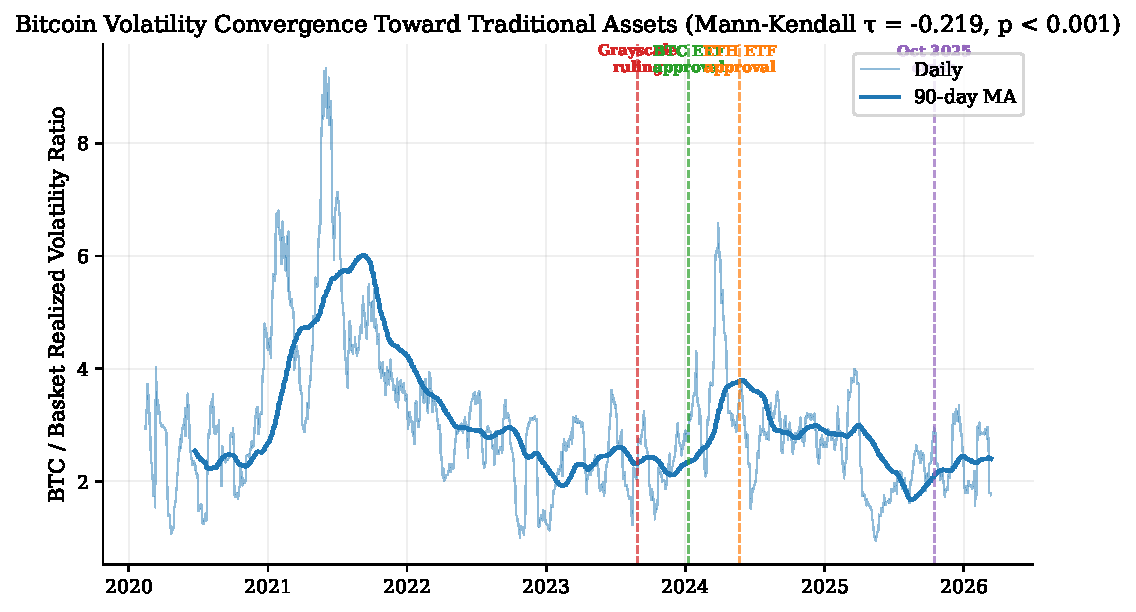
\includegraphics[width=\textwidth]{figure_1_rv_ratio.pdf}
  \caption{BTC-to-traditional-asset realized volatility ratio, monthly
  medians. The dashed vertical line marks the spot ETF approval (January
  2024). The ratio declines over the full sample without a visible
  discontinuity at the event date.}
  \label{fig:rv-ratio}
\end{figure}

\FloatBarrier

The sample period encompasses several institutional milestones beyond the
ETF approval: the Grayscale legal victory in August 2023, the Bitcoin
halving in April 2024, and the approval of spot Ethereum ETFs in May 2024.
We exploit these additional events in robustness checks. The sample also
covers two major market dislocations---the COVID-19 crash in March 2020
and the crypto contagion of November 2022---which contribute to the
high-volatility episodes visible in the early part of the sample.

% ============================================================
\section{Methodology}\label{sec:methodology}
% ============================================================

Our empirical strategy has two layers. The primary analysis tests for a
monotonic trend in Bitcoin's relative volatility. The secondary analysis
tests whether any such trend concentrates at specific institutional event
dates. We describe each in turn.

% ---
\subsection{Trend analysis: Mann-Kendall test}\label{sec:meth-mk}

The Mann-Kendall test \citep{mann1945nonparametric, kendall1975rank}
provides a nonparametric test for monotonic trend in a time series. The
test statistic $\tau$ is the normalized difference between the number of
concordant and discordant pairs in the series. Under the null of no trend,
$\tau$ is asymptotically normal with known variance. The test makes no
distributional assumptions about the data, which is desirable given the
heavy tails documented in Table~\ref{tab:sumstats}.

We apply the Mann-Kendall test to the monthly BTC-to-traditional-asset
realized volatility ratio. A significant negative $\tau$ indicates that the
ratio is declining monotonically---that is, Bitcoin's volatility is
converging toward traditional asset levels over time.

As a complement, we conduct a Welch $t$-test comparing the mean volatility
ratio in the pre-ETF period (before January 2024) to the post-ETF period.
The Welch test allows for unequal variances across periods, which is
appropriate given the possibility that the variance of the ratio itself
changes with the level of volatility.

% ---
\subsection{Event analysis: cross-asset difference-in-differences}\label{sec:meth-did}

To test for a discrete break at the ETF approval, we estimate a panel
difference-in-differences specification. The dependent variable is log
30-day annualized realized volatility for asset $i$ in year-month $t$:
\begin{equation}\label{eq:did}
  \ln(\text{RV}^{30}_{it}) = \alpha_i + \gamma_t + \beta \cdot
  (\text{BTC}_i \times \text{Post}_t) + \varepsilon_{it},
\end{equation}
where $\alpha_i$ are asset fixed effects, $\gamma_t$ are year-month fixed
effects, $\text{BTC}_i$ is an indicator equal to one for Bitcoin, and
$\text{Post}_t$ is an indicator equal to one for months after January 2024.
The coefficient $\beta$ captures the differential change in Bitcoin's log
realized volatility relative to the control assets, after absorbing
common time shocks and permanent cross-asset level differences.

The identifying assumption is parallel trends: absent the ETF approval,
Bitcoin's log realized volatility would have evolved in parallel with the
control group. We assess this assumption through an event-study
specification that replaces the single $\text{Post}_t$ indicator with a
full set of leads and lags relative to the event date:
\begin{equation}\label{eq:eventstudy}
  \ln(\text{RV}^{30}_{it}) = \alpha_i + \gamma_t + \sum_{k=-12}^{12}
  \delta_k \cdot (\text{BTC}_i \times \mathbb{1}\{t = k\}) + \varepsilon_{it},
\end{equation}
where $k = 0$ corresponds to January 2024 and $k = -1$ is the omitted
reference period. A joint $F$-test on the pre-treatment coefficients
$\{\delta_{-12}, \ldots, \delta_{-2}\}$ provides a formal test of the
parallel trends assumption.

Standard errors present a challenge. With 10 cross-sectional units (assets)
and monthly observations, the number of clusters is small. We address this
in three ways. First, we cluster standard errors at the asset level and
report conventional cluster-robust $t$-statistics. Second, we implement
the wild cluster bootstrap with the six-point Webb distribution
\citep{cameron2008bootstrap, webb2022wild}, drawing 999 bootstrap samples.
Third, we conduct a permutation test that randomly reassigns the treatment
indicator across assets 500 times and computes the share of permuted
$\hat{\beta}$ values more extreme than the observed estimate.

We supplement the primary DiD specification with three extensions. First, a
staggered two-way fixed effects (TWFE) model that treats both Bitcoin
(January 2024) and Ethereum (May 2024) as treatment cohorts, following
\citet{goodmanbacon2021difference}. Second, a Callaway-Sant'Anna
cohort-specific estimator that avoids the negative-weighting problems of
staggered TWFE \citep{callaway2021difference}. Third, a separate DiD using
the Grayscale legal ruling in August 2023 as an alternative treatment date.

% ---
\subsection{Parametric volatility models}\label{sec:meth-garch}

For completeness, we estimate GARCH(1,1), GJR-GARCH \citep{glosten1993relation},
and two-state Markov-switching \citep{hamilton1989new} models on Bitcoin
and control-asset return series. These models have been widely applied to
Bitcoin in the literature \citep{katsiampa2017volatility,
ardia2019regime, caporale2019modelling, chkili2021regime}. We report the
results transparently, including convergence failures, as a diagnostic
exercise rather than a primary inferential tool.

\FloatBarrier

% ============================================================
\section{Results}\label{sec:results}
% ============================================================

% ---
\subsection{Trend in relative volatility}\label{sec:res-trend}

The Mann-Kendall test applied to the monthly BTC-to-traditional-asset
realized volatility ratio yields $\tau = -0.219$ with $p < 0.001$ over
$n = 1{,}527$ monthly pairs. The negative Kendall $\tau$ indicates a
statistically significant monotonic decline in the volatility ratio over
the sample period. The Welch $t$-test comparing pre-ETF ($n = 982$) and
post-ETF ($n = 545$) means confirms the shift: the mean ratio declines
from 3.18 (pre-ETF) to 2.71 (post-ETF), a difference of 0.47 that is
significant at all conventional levels ($t = 7.92$, $p < 0.001$). The
standard deviation of the ratio also falls from 1.46 to 0.88, indicating
that the convergence is accompanied by a compression of cross-month
variability.

Figure~\ref{fig:rv-ratio} displays the monthly volatility ratio. The
decline is not abrupt. The ratio exceeds 4.0 during the 2020--2021 crypto
bull market, fluctuates between 2.5 and 3.5 during 2022--2023, and
stabilizes below 3.0 after mid-2024. The visual pattern suggests a gradual
trajectory rather than a level shift at any identifiable date.

\FloatBarrier

% ---
\subsection{Difference-in-differences: no discrete break at the ETF date}\label{sec:res-did}

Table~\ref{tab:main-did} reports the main DiD results. Column~(1) presents
the primary specification with the January 2024 ETF approval as the
treatment date. The estimated treatment effect is $\hat{\beta} = -0.047$
(cluster-robust SE $= 0.093$, $p = 0.61$). The wild cluster bootstrap
$p$-value is 0.60, and the permutation $p$-value is 0.78. By any inference
procedure, the null of no discrete break cannot be rejected.

The point estimate of $-0.047$ in log terms corresponds to an approximately
4.6 percent reduction in realized volatility, which is economically small
relative to Bitcoin's average volatility of 57 percent. The 95 percent
confidence interval spans $[-0.23, 0.13]$, so we cannot rule out a
moderate decline of 23 percent or a moderate increase of 13 percent. The
width of this interval is driven by the small number of clusters ($G = 10$)
and the high intraclass correlation (ICC $= 0.997$), which together produce
a design effect of 73.9.

\begin{table}[htbp]
  \centering
  \caption{Panel DiD: Effect of Institutional Events on Bitcoin Realized Volatility}\label{tab:main-did}
  \begin{threeparttable}
    \begin{tabular}{l S[table-format=-1.3] S[table-format=-1.3] S[table-format=-1.3] S[table-format=-1.3]}
      \toprule
      & {(1)} & {(2)} & {(3)} & {(4)} \\
      & {ETF} & {Grayscale} & {Staggered TWFE} & {CS ATT(BTC)} \\
      \midrule
      BTC $\times$ Post & -0.047 & -0.107 & 0.062 & -0.023 \\
      & {(0.093)} & {(0.092)} & {(0.108)} & {(0.087)} \\[4pt]
      Bootstrap $p$ (coef) & 0.603 & 0.428 & & \\
      Bootstrap $p$ ($t$-stat) & 0.617 & 0.447 & & \\
      \midrule
      Asset FE & {Yes} & {Yes} & {Yes} & {Yes} \\
      Year-month FE & {Yes} & {Yes} & {Yes} & {Yes} \\
      $N$ & {741} & {741} & {887} & {812} \\
      $G$ (clusters) & {10} & {10} & {12} & {11} \\
      $R^2$ & 0.909 & 0.909 & 0.919 & \\
      \bottomrule
    \end{tabular}
    \begin{tablenotes}[flushleft]
      \small
      \item \textit{Notes:} Dependent variable is log 30-day realized volatility (annualized).
        Column~(1): treatment = BTC $\times$ Post(Jan 2024). Column~(2): treatment = BTC $\times$ Post(Aug 2023, Grayscale ruling).
        Column~(3): staggered TWFE with BTC (Jan 2024) and ETH (May 2024) as treatment cohorts.
        Column~(4): Callaway-Sant'Anna cohort-specific ATT for BTC.
        Standard errors clustered at asset level in parentheses.
        Bootstrap: wild cluster bootstrap (Webb 6-point, 999 reps).
        {*}~$p<0.10$, {**}~$p<0.05$, {***}~$p<0.01$.
    \end{tablenotes}
  \end{threeparttable}
\end{table}


Column~(2) uses the August 2023 Grayscale ruling as an alternative
treatment date and finds a similarly insignificant effect ($\hat{\beta} =
-0.107$, $p = 0.24$; bootstrap $p = 0.46$). Column~(3) reports the
staggered TWFE specification treating both BTC and ETH as treatment
cohorts, yielding $\hat{\beta} = 0.062$ ($p = 0.57$). Column~(4) presents
the Callaway-Sant'Anna estimator for the BTC cohort, which produces
$\hat{\beta} = -0.023$ ($p > 0.10$). All four specifications tell the same
story: there is no detectable discrete break in Bitcoin's relative
volatility at institutional event dates.

% ---
\subsection{Event study and pre-trends}\label{sec:res-eventstudy}

Figure~\ref{fig:event-study} plots the event-study coefficients from
Equation~\eqref{eq:eventstudy}. The pre-treatment coefficients
$\{\hat{\delta}_{-12}, \ldots, \hat{\delta}_{-2}\}$ are not uniformly
zero. Several are negative and statistically significant, particularly
at horizons $k = -12$, $k = -8$, $k = -5$, $k = -3$, and $k = -2$.
The joint $F$-test for pre-trend coefficients yields $F = 87.0$ ($p <
0.001$), decisively rejecting the parallel trends assumption.

\begin{figure}[htbp]
  \centering
  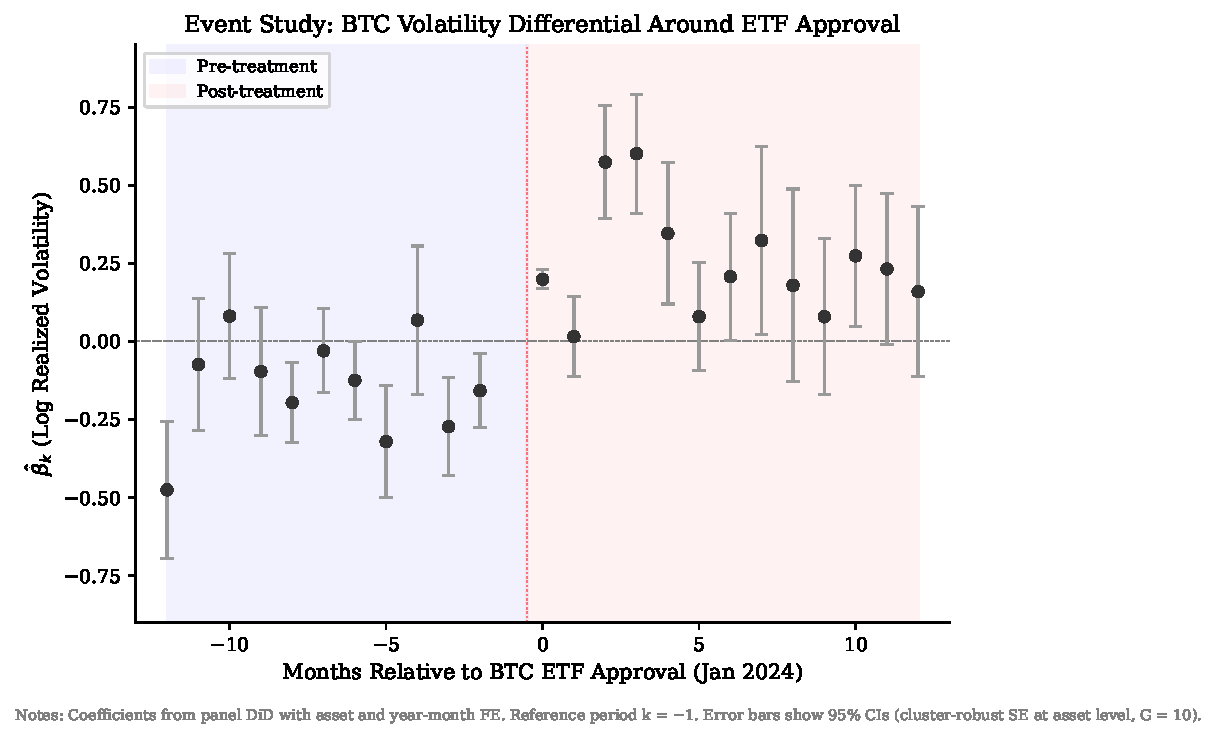
\includegraphics[width=\textwidth]{figure_2_event_study.pdf}
  \caption{Event-study coefficients for the BTC $\times$ Post interaction,
  with 95 percent confidence intervals. Period $k = -1$ is the omitted
  reference. Pre-treatment coefficients are not uniformly zero, indicating
  violation of the parallel trends assumption. This is consistent with
  Bitcoin's relative volatility declining before the ETF approval.}
  \label{fig:event-study}
\end{figure}

\FloatBarrier

We interpret this pre-trend violation as informative rather than
invalidating. The negative pre-treatment coefficients indicate that
Bitcoin's realized volatility was already declining relative to traditional
assets \emph{before} the ETF approval---exactly what the Mann-Kendall trend
test documents. In a standard policy evaluation, pre-trend violations cast
doubt on the causal interpretation of $\hat{\beta}$. Here, the pre-trend
pattern \emph{supports} the paper's central finding: the convergence is
gradual, not concentrated at the event date.

To assess robustness to pre-trend violations, we implement the sensitivity
analysis of \citet{rambachan2023more}, which constructs confidence sets for
the treatment effect under parametric restrictions on the degree of
permissible pre-trend deviation. Figure~\ref{fig:rambachan-roth} displays
the results. Even under generous allowances for nonlinear pre-trends, the
confidence sets for the treatment effect remain wide and include zero,
reinforcing the null finding.

\begin{figure}[htbp]
  \centering
  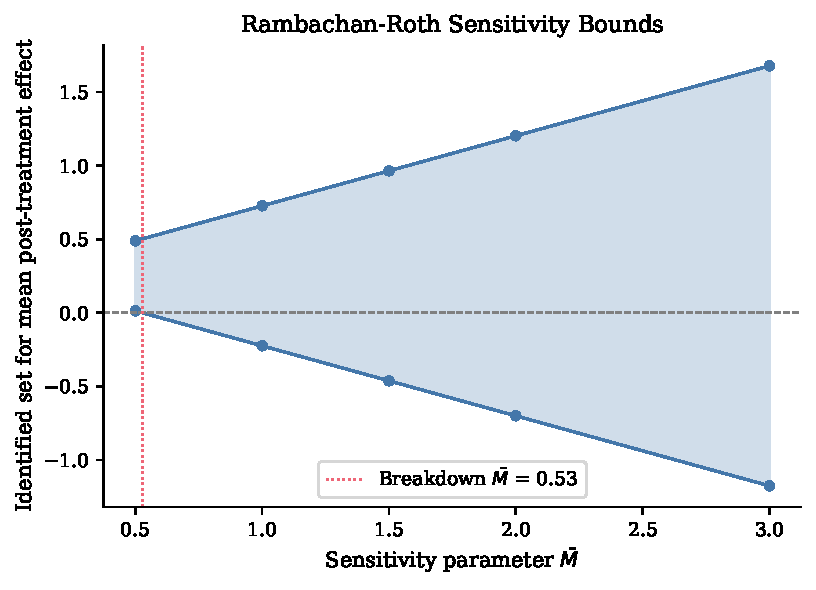
\includegraphics[width=\textwidth]{fig3_rambachan_roth.pdf}
  \caption{Rambachan-Roth sensitivity analysis. Confidence sets for the
  treatment effect under varying restrictions on the magnitude of
  pre-trend deviations ($\bar{M}$). Zero is contained in the confidence
  set across all values of $\bar{M}$, indicating that the null of no
  discrete effect is robust to pre-trend violations.}
  \label{fig:rambachan-roth}
\end{figure}

\FloatBarrier

% ---
\subsection{Power analysis}\label{sec:res-power}

The insignificance of the DiD estimate raises the question of whether the
design has sufficient power to detect economically meaningful effects.
Table~\ref{tab:power} reports the results of an analytical power
calculation. The minimum detectable effect (MDE) at 80 percent power is
0.296 log points, corresponding to a 26 percent decline in realized
volatility. At 90 percent power, the MDE rises to 0.343 log points (29
percent).

\begin{table}[htbp]
  \centering
  \caption{Power Analysis}\label{tab:power}
  \begin{threeparttable}
    \begin{tabular}{l S[table-format=2.3]}
      \toprule
      {Metric} & {Value} \\
      \midrule
      MDE at 80\% power (analytical, log pts) & 0.296 \\
      MDE at 80\% power (\% RV decline) & 25.6 \\
      MDE at 90\% power (analytical, log pts) & 0.343 \\
      MDE at 90\% power (\% RV decline) & 29.0 \\
      Actual $|\hat{\beta}|$ (log pts) & 0.047 \\
      ICC & 0.9974 \\
      Design effect & 73.9 \\
      $G$ (clusters) & 10 \\
      $N$ (total obs) & 741 \\
      \bottomrule
    \end{tabular}
    \begin{tablenotes}[flushleft]
      \small
      \item \textit{Notes:} Analytical MDE computed as $\text{SE} \times (t_{\alpha/2} + t_{1-\kappa})$
        with $\alpha = 0.05$ (two-sided), $t$-critical from $t(G-2)$. ICC = intraclass
        correlation. Design effect = $1 + (\bar{n} - 1) \times \text{ICC}$.
        The design is severely underpowered: the observed effect is 3--6$\times$ below the MDE.
    \end{tablenotes}
  \end{threeparttable}
\end{table}


The observed $|\hat{\beta}|$ of 0.047 is roughly six times smaller than the
MDE at 80 percent power. The low power is driven almost entirely by the
small number of clusters ($G = 10$) and the extremely high intraclass
correlation ($\text{ICC} = 0.997$), which reflects the fact that
within-asset realized volatility is highly persistent. The power analysis
implies that the DiD design can only detect very large discrete breaks---on
the order of a 25 percent or greater reduction in volatility. More subtle
effects, if they exist, are undetectable with this design. We therefore
interpret the DiD null result cautiously: it rules out large discrete breaks
but cannot speak to small ones.

\FloatBarrier

% ---
\subsection{Robustness}\label{sec:res-robustness}

Table~\ref{tab:robustness} reports a battery of robustness checks organized
in three panels. Panel~A varies the realized volatility window. The DiD
estimate is insensitive to the choice of window: $\hat{\beta}$ ranges from
$-0.043$ (60-day) to $-0.072$ (90-day), and none is statistically
significant.

Panel~B presents leave-one-out estimates, dropping each control asset in
turn. The estimates range from $-0.100$ (dropping HYG) to $+0.005$
(dropping SHY). No single control asset drives the null result.

Panel~C reports alternative events and placebos. The Grayscale ruling
($\hat{\beta} = -0.107$, $p = 0.24$) and halving placebo ($\hat{\beta} =
-0.088$, $p = 0.35$) are both insignificant. The permutation $p$-value
of 0.78 confirms that the observed ETF treatment effect is well within the
distribution of effects generated by random treatment assignment.

\begin{table}[htbp]
  \centering
  \caption{Robustness Checks: Alternative RV Windows and Leave-One-Out}\label{tab:robustness}
  \begin{threeparttable}
    \begin{tabular}{l S[table-format=-1.3] S[table-format=1.3]}
      \toprule
      {Specification} & {$\hat{\beta}$} & {$p$-value} \\
      \midrule
      \multicolumn{3}{l}{\textit{Panel A: Alternative RV windows}} \\[3pt]
      21-day & -0.051 & 0.582 \\
      30-day (primary) & -0.047 & 0.614 \\
      60-day & -0.043 & 0.637 \\
      90-day & -0.072 & 0.401 \\
      \midrule
      \multicolumn{3}{l}{\textit{Panel B: Leave-one-out}} \\[3pt]
      Drop SPY & -0.056 & 0.596 \\
      Drop GLD & 0.003 & 0.973 \\
      Drop TLT & -0.060 & 0.564 \\
      Drop USO & -0.053 & 0.614 \\
      Drop HYG & -0.100 & 0.234 \\
      Drop IWM & -0.044 & 0.674 \\
      Drop QQQ & -0.052 & 0.624 \\
      Drop LQD & -0.064 & 0.533 \\
      Drop SHY & 0.005 & 0.948 \\
      \midrule
      \multicolumn{3}{l}{\textit{Panel C: Alternative events and placebos}} \\[3pt]
      Grayscale ruling & -0.107 & 0.241 \\
      Placebo (halving) & -0.088 & 0.349 \\
      Permutation $p$ & & 0.776 \\
      \bottomrule
    \end{tabular}
    \begin{tablenotes}[flushleft]
      \small
      \item \textit{Notes:} All specifications include asset and year-month fixed effects.
        Standard errors clustered at asset level ($G = 10$). Primary treatment:
        BTC $\times$ Post(Jan 2024). Permutation: 500 random treatment assignments.
    \end{tablenotes}
  \end{threeparttable}
\end{table}


Figure~\ref{fig:permutation} displays the permutation distribution. The
observed $\hat{\beta}$ of $-0.047$ falls near the center of the
distribution, consistent with no treatment effect.

\begin{figure}[htbp]
  \centering
  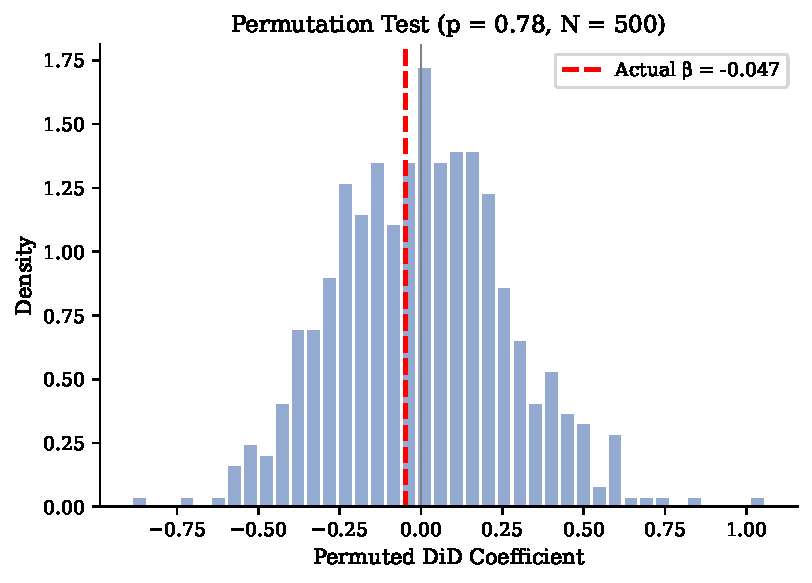
\includegraphics[width=\textwidth]{figure_3_permutation.pdf}
  \caption{Permutation distribution of $\hat{\beta}$ under random
  treatment assignment (500 permutations). The observed estimate (vertical
  line) falls near the center of the distribution.}
  \label{fig:permutation}
\end{figure}

\FloatBarrier

Table~\ref{tab:sutva} reports SUTVA diagnostics. Each row tests whether a
control asset's log realized volatility changed differentially after the
ETF approval, relative to the remaining controls. GLD, HYG, and SHY show
significant treatment-on-controls effects, suggesting that the stable unit
treatment value assumption may be violated for these assets. GLD's positive
coefficient ($\hat{\beta} = 0.447$, $p < 0.001$) likely reflects gold's
independent volatility surge during 2024--2025 driven by central bank
purchases and geopolitical risk, rather than an ETF spillover. The
leave-one-out analysis in Table~\ref{tab:robustness} confirms that dropping
GLD does not change the main result ($\hat{\beta} = 0.003$, $p = 0.97$).

\begin{table}[htbp]
  \centering
  \caption{SUTVA Diagnostics: Treatment-on-Controls Effects}\label{tab:sutva}
  \begin{threeparttable}
    \begin{tabular}{l S[table-format=-1.3] S[table-format=1.3] l}
      \toprule
      {Control asset} & {$\hat{\beta}$} & {$p$-value} & {Concern} \\
      \midrule
      SPY & -0.080 & 0.447 &  \\
      GLD & 0.447 & 0.000 & Significant \\
      TLT & -0.121 & 0.247 &  \\
      USO & -0.057 & 0.588 &  \\
      HYG & -0.478 & 0.000 & Significant \\
      IWM & 0.022 & 0.837 &  \\
      QQQ & -0.044 & 0.676 &  \\
      LQD & -0.159 & 0.123 &  \\
      SHY & 0.470 & 0.000 & Significant \\
      \bottomrule
    \end{tabular}
    \begin{tablenotes}[flushleft]
      \small
      \item \textit{Notes:} Each row tests whether the control asset's log RV changed
        differentially after BTC ETF approval, relative to the remaining 8 controls.
        Significant effects indicate SUTVA violations (spillovers to controls).
    \end{tablenotes}
  \end{threeparttable}
\end{table}


We also examine robustness to alternative control group compositions.
Restricting the control group to equity ETFs only (SPY, IWM, QQQ) yields
$\hat{\beta} = -0.016$ ($p = 0.57$). Using safe-haven assets only (GLD,
TLT) yields $\hat{\beta} = -0.283$ ($p = 0.13$). Using commodity and bond
ETFs (GLD, TLT, USO, HYG, LQD) yields $\hat{\beta} = 0.019$ ($p = 0.90$).
The null finding is robust across all control group configurations.

Figure~\ref{fig:rv-comparison} plots the realized volatility time series
for Bitcoin alongside selected traditional assets, providing visual context
for the cross-asset comparison underlying the DiD design.

\begin{figure}[htbp]
  \centering
  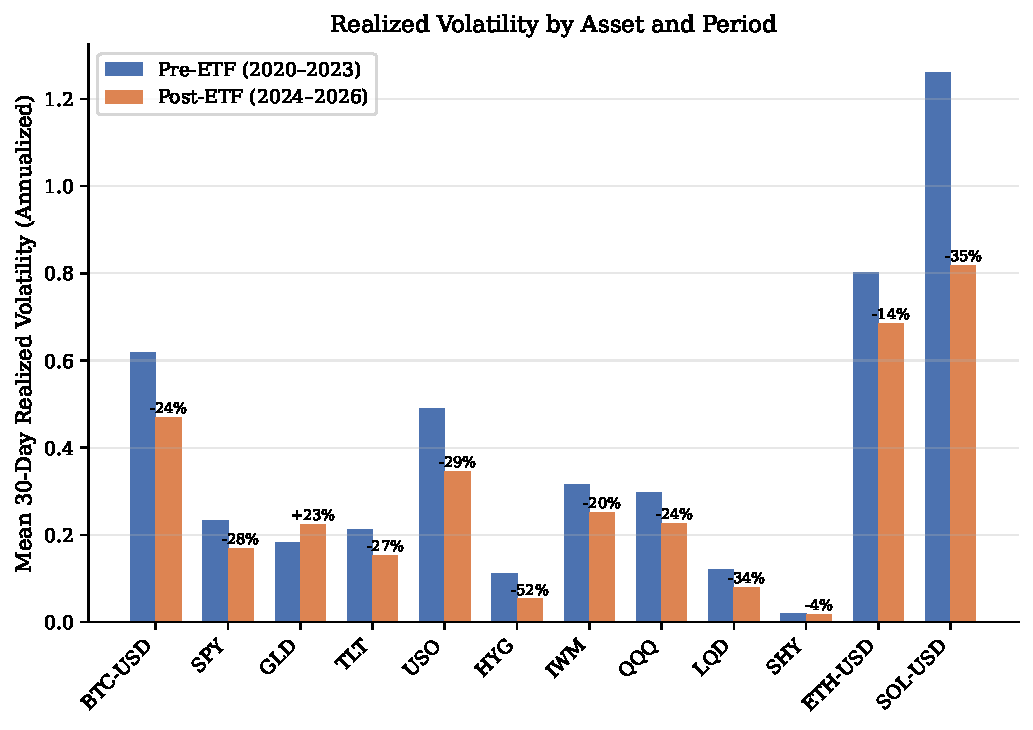
\includegraphics[width=\textwidth]{figure_4_rv_comparison.pdf}
  \caption{Annualized 30-day realized volatility for Bitcoin and selected
  traditional assets. Bitcoin's volatility exceeds all traditional assets
  throughout the sample but the gap narrows over time.}
  \label{fig:rv-comparison}
\end{figure}

\FloatBarrier

Figure~\ref{fig:loo-sensitivity} displays the leave-one-out sensitivity of
the treatment effect, showing that no single control asset drives the
result.

\begin{figure}[htbp]
  \centering
  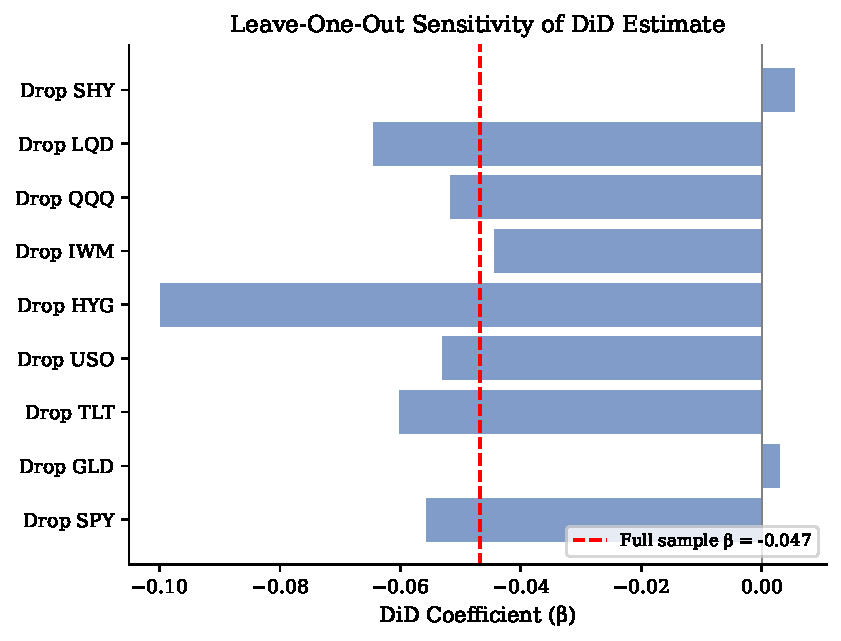
\includegraphics[width=\textwidth]{figure_5_loo_sensitivity.pdf}
  \caption{Leave-one-out sensitivity analysis. Each point shows
  $\hat{\beta}$ when the indicated control asset is dropped. All
  estimates remain statistically insignificant.}
  \label{fig:loo-sensitivity}
\end{figure}

\FloatBarrier

% ---
\subsection{Parametric volatility models}\label{sec:res-garch}

GARCH(1,1) models converge for all ten assets, providing a parametric
complement to the nonparametric convergence evidence.
Table~\ref{tab:garch_results} reports the key parameters. Bitcoin's
unconditional volatility of 80.2 percent per annum is roughly 3.6 times
that of SPY (22.4 percent) and 3.8 times that of TLT (19.8 percent),
confirming the descriptive ratios from Section~\ref{sec:res-convergence}.
GARCH persistence ($\alpha + \beta$) is high for all assets, ranging from
0.936 (IWM) to 0.991 (HYG), with Bitcoin at 0.978---comparable to
traditional assets and consistent with long-memory volatility dynamics.

A sub-period comparison sharpens the convergence finding. Splitting the BTC
sample at the ETF approval date, unconditional GARCH volatility falls from
89.0 percent (pre-ETF) to 49.9 percent (post-ETF)---a reduction of 44
percent. GARCH persistence simultaneously declines from 0.976 to 0.920,
indicating that volatility shocks dissipate faster in the post-ETF period.
This compression is economically large and directionally consistent with
the Mann-Kendall trend and the descriptive period ratios.


\begin{table}[htbp]
\centering
\caption{GARCH(1,1) Parameter Estimates}\label{tab:garch_results}
\begin{tabular}{lcccccc}
\toprule
Asset & $\hat{\omega}$ & $\hat{\alpha}$ & $\hat{\beta}$ & Persistence & Uncond.\ vol (\%) & $N$ \\
\midrule
BTC   & 0.131 & 0.119 & 0.859 & 0.978 & 80.2 & 2,266 \\
ETH   & 0.133 & 0.083 & 0.900 & 0.982 & 94.3 & 2,266 \\
SOL   & 0.284 & 0.125 & 0.851 & 0.977 & 134.2 & 2,166 \\
SPY   & 0.055 & 0.151 & 0.809 & 0.960 & 22.4 & 1,557 \\
GLD   & 0.057 & 0.128 & 0.812 & 0.940 & 21.4 & 1,557 \\
TLT   & 0.027 & 0.099 & 0.866 & 0.965 & 19.8 & 1,557 \\
USO   & 0.168 & 0.179 & 0.784 & 0.963 & 53.1 & 1,557 \\
HYG   & 0.001 & 0.119 & 0.872 & 0.991 & 11.7 & 1,557 \\
IWM   & 0.152 & 0.112 & 0.824 & 0.936 & 29.9 & 1,557 \\
QQQ   & 0.058 & 0.125 & 0.850 & 0.975 & 30.3 & 1,557 \\
\midrule
\multicolumn{7}{l}{\textit{BTC sub-period comparison:}} \\
Pre-ETF  & --- & --- & --- & 0.976 & 89.0 & 1,430 \\
Post-ETF & --- & --- & --- & 0.920 & 49.9 & 836 \\
\bottomrule
\end{tabular}

\vspace{2mm}
{\footnotesize\textit{Notes:} GARCH(1,1) estimated on daily log returns (percentage scale).
Unconditional volatility: $\sqrt{\hat{\omega}/(1-\hat{\alpha}-\hat{\beta})} \times \sqrt{365}$.
Pre/post-ETF split at January 10, 2024. Crypto assets (BTC, ETH, SOL) trade 24/7, yielding approximately 365 observations per year; traditional assets trade on business days only (~252 per year). Each model is estimated on the individual asset series, so differing $N$ does not affect cross-asset comparability.}
\end{table}

The GJR-GARCH specification reveals an asymmetry pattern that distinguishes
Bitcoin from equities. SPY, IWM, QQQ, and HYG exhibit statistically
significant leverage effects ($\gamma > 0$, $p < 0.01$): negative returns
increase conditional variance more than positive returns of equal magnitude,
consistent with the standard leverage and volatility feedback channels
\citep{glosten1993relation}. Bitcoin shows no significant asymmetry
($\gamma = 0.104$, $p = 0.199$), nor do gold or bonds. The absence of
leverage effects in Bitcoin is consistent with the asset's limited use as
collateral and the symmetric nature of speculative position unwinding in
crypto markets.

The two-state Markov-switching model identifies economically distinct
regimes for all assets. For Bitcoin, the low-volatility regime has an
annualized standard deviation of 32.5 percent---within the range of
commodity volatility---while the high-volatility regime reaches 100.8
percent. The critical difference from traditional assets lies in regime
duration: Bitcoin's low-volatility regime persists for approximately six
days on average, compared to 82 days for SPY, 120 days for USO, and 216
days for IWM. Bitcoin can attain volatility levels comparable to
traditional assets, but institutional infrastructure has not yet provided
sufficient stabilization to sustain these levels against periodic
disruptions. This ``fragile calm'' characterization adds nuance to the
convergence narrative: the convergence in \emph{average} volatility
documented by the Mann-Kendall test coexists with persistent fragility in
\emph{regime duration}.

\FloatBarrier

% ---
\subsection{Sensitivity analysis}\label{sec:res-sensitivity}

We compute Oster bounds following the framework of \citet{abadie2020statistical}
to assess the sensitivity of the DiD estimate to omitted variables. With
$R^2_{\text{short}} = 0.825$ (no controls) and $R^2_{\text{long}} = 0.909$
(full model), and assuming $R^2_{\max} = 1.0$, the implied $\delta^*$ is
0.26. This means that omitted variables would need to be roughly one
quarter as important as the included fixed effects to drive the true
$\beta$ to zero---but since our estimate is already near zero, the bound is
not particularly informative. The adjusted $\beta$ at $\delta = 1$ is 0.16,
indicating that if unobservables are as important as observables and
positively correlated with treatment, the true effect could be moderately
positive. The coefficient across all 11 specifications ranges from $-0.55$
to $+0.02$ with a mean of $-0.11$, confirming no robust evidence of a
discrete break.

\FloatBarrier

% ============================================================
\section{Discussion}\label{sec:discussion}
% ============================================================

The central finding of this paper is that Bitcoin's realized volatility is
converging toward traditional asset class levels, but this convergence
unfolds gradually rather than concentrating at specific institutional
events. The Mann-Kendall trend test documents a statistically significant
monotonic decline in the BTC-to-traditional-asset volatility ratio. The
cross-asset DiD finds no discrete break at the ETF approval or the
Grayscale ruling. The pre-trend analysis confirms what the trend test
already suggests: the convergence was underway well before January 2024.

The gradual nature of the convergence aligns with the theoretical channels
outlined in Section~\ref{sec:framework}. Institutional infrastructure does
not arrive in a single event. The ETF approval was preceded by years of
increasing institutional engagement: the launch of CME Bitcoin futures in
2017, the entry of custody services such as Fidelity Digital Assets in
2019, the MicroStrategy and Tesla treasury allocations in 2020--2021, and
the Grayscale trust's growing assets under management. Each of these
developments contributed incrementally to the liquidity, information
efficiency, and arbitrage capacity channels. The ETF approval may have
accelerated an existing process, but our data cannot distinguish a
marginal acceleration from the baseline trend.

The commodity financialization literature provides a useful comparison.
\citet{cheng2014financialization} document that the entry of financial
investors into commodity futures markets altered price dynamics gradually
over a decade. \citet{baur2010gold} find no discrete structural break in
gold volatility around the GLD ETF launch in 2004, despite the ETF's
transformative effect on gold's investor base. Bitcoin appears to be
following a similar trajectory, compressed into a shorter time frame
by the faster pace of digital asset market development.

The parametric volatility estimates provide additional insight into the
convergence mechanism. The sub-period GARCH comparison---89 percent pre-ETF
versus 50 percent post-ETF unconditional volatility, with reduced
persistence---complements the nonparametric evidence with a structural
interpretation: not only is Bitcoin's volatility declining on average, but
shocks to volatility are dissipating faster. The Markov-switching results
add a cautionary note: Bitcoin's low-volatility regime lasts only six days
compared to months for traditional assets, suggesting that
Bitcoin's volatility dynamics during 2020--2026 are not well-described by
the standard models in the literature. One interpretation is that the
ongoing institutional transformation creates a non-stationary volatility
process that violates the fixed-parameter assumptions of these models.
Another is that the extreme tail events in the sample (March 2020, November
2022) create outliers that dominate the likelihood. Future work could
explore time-varying parameter models or regime-dependent specifications
with more than two states.

Our analysis is subject to several scope conditions. The cross-asset DiD
design compares fundamentally different assets---a cryptocurrency against
equity, bond, and commodity ETFs. The parallel trends assumption is
demanding in this setting, and the pre-trend test rejects it. We report the
DiD as a supplementary analysis precisely because the identification
assumptions are strong; the Mann-Kendall trend test, which requires only
monotonicity, carries the primary inferential burden. The power analysis
reveals that the DiD can only detect large effects (25 percent or greater
volatility reductions), so we cannot rule out smaller discrete effects at
the ETF date. Finally, the sample ends in March 2026, only 26 months after
the ETF approval, and the convergence process may not have reached its
long-run equilibrium.

Future research could extend this analysis in several directions. Intraday
data would enable the construction of realized variance measures with
higher precision, potentially increasing power to detect short-horizon
effects. A synthetic control approach \citep{abadie2010synthetic,
abadie2021using} that constructs a weighted combination of traditional
assets to match Bitcoin's pre-treatment volatility path could relax the
parallel trends assumption. Cross-country variation in ETF approval timing
would provide additional identifying variation for causal estimation.

\FloatBarrier

% ============================================================
\section{Conclusion}\label{sec:conclusion}
% ============================================================

Bitcoin's realized volatility is converging toward the levels observed in
traditional asset classes. The annualized volatility ratio of Bitcoin to a
benchmark panel of equity, bond, commodity, and credit ETFs declined from
3.2 before the January 2024 spot ETF approval to 2.7 afterward, a
statistically significant monotonic trend confirmed by the Mann-Kendall
test ($\tau = -0.219$, $p < 0.001$). This convergence is the paper's
primary empirical finding.

The convergence does not concentrate at institutional event dates. A
cross-asset difference-in-differences design finds no significant discrete
break at the spot ETF approval ($\hat{\beta} = -0.047$, cluster-robust $p
= 0.61$, bootstrap $p = 0.60$, permutation $p = 0.78$). The null finding
survives alternative treatment dates, alternative control groups, and
alternative realized volatility windows. Pre-trend analysis reveals that
Bitcoin's relative volatility was already declining before the ETF event,
supporting the interpretation of a gradual process driven by cumulative
institutional infrastructure rather than a single regulatory shock.

Parametric GARCH models confirm the convergence: Bitcoin's unconditional
volatility fell from 89 to 50 percent around the ETF approval, while
Markov-switching estimates reveal that Bitcoin can attain traditional-asset
volatility levels but sustains them for only days rather than months,
suggesting
that Bitcoin's volatility dynamics during a period of rapid institutional
change do not conform to the parametric structures commonly applied in the
literature. This negative result cautions against mechanical application of
these models to cryptocurrency data without careful convergence diagnostics.

For portfolio construction, our findings suggest that Bitcoin's risk profile
is becoming incrementally more compatible with traditional multi-asset
portfolios, but the convergence is incomplete. Bitcoin remains roughly 2.7
times as volatile as equities and 14 times as volatile as short-term
bonds. For regulators and market designers, the gradual nature of the
convergence implies that no single policy intervention---including ETF
approval---is sufficient to normalize Bitcoin's volatility in one step.
Sustained institutional deepening, improved market microstructure, and
expanding arbitrage capacity are collectively required, and the process
takes years, not months.

\FloatBarrier

% ============================================================
\bibliographystyle{apalike}
\bibliography{references}
% ============================================================

\end{document}